\section{Theorie}
\label{sec:Theorie}

\subsection{Fehlerrechnung}

Für die Fehlerfortpflanzung bei Gleichungen mit $N$ fehlerbehafteten Größen
wird jeweils die Formel zur Gaußschen Fehlerfortpflanzung

\begin{equation*}
  \sigma = \sqrt{\sum_{i=1}^{N}\biggl(\frac{\partial f(x_{\g{i}})}{\partial x_{\g{i}}}
  \sigma_{\g{i}}\biggr)^2}
\end{equation*}
mit der jeweiligen Funktion $f(x_{\g{i}})$, den Messgrößen $x_{\g{i}}$ und den
zugehörigen Fehlern $\sigma_i$ verwendet.
Zur Berechnung des arithmetischen Mittels von $N$ Messwerten wird jeweils die
Formel

\begin{equation*}
  \bar{x} = \frac{1}{N}\sum_{i=1}^{N}x_{\g{i}}
\end{equation*}
mit den Messwerten $x_i$ benutzt.
Die Standardabweichung des Mittelwerts wird jeweils mit der Gleichung

\begin{equation*}
  \bar{\sigma} = \sqrt{\frac{1}{N-1}\sum_{i=1}^{N}(x_{\g{i}} - \bar{x})^2}
\end{equation*}
mit den $N$ Messwerten $x_i$ berechnet.

\subsection{Einleitung}

Der Photoeffekt beschreibt die Auslösung von Elektronen aus einer
Metalloberfläche durch Bestrahlung mit Licht. Hierbei treten verschiedene Effekte wie
die Auslöseabhängigkeit von der Frequenz des Lichts auf. Zur Erklärung dieser Effekte muss zunächst
die Gestalt des Lichts geklärt werden.

\subsection{Gestalt des Lichts}

Bei der Beobachtung der verschiedenen Effekte von Licht
treten zwei scheinbar gegensätzliche Theorien auf: die Wellentheorie und die
Korpuskeltheorie. Die Wellentheorie beschreibt Erscheinungen wie Beugung und Interferenz,
wohingegen die Korpuskeltheorie Beobachtungen bei der Wechselwirkung
mit Materie erklärt.
Die Quantenelektrodynamik kann alle diese Effekte erklären und hat die beiden
vorher erwähnten Theorien als Grenzfälle.

Also werden alle Effekte bei denen viele Photonen beteiligt sind mit
der Wellentheorie beschrieben und zur Erklärung der Wechselwirkungen mit Materie
wird die Quantelung des Lichts benutzt.

\subsection{Phänomene beim Photoeffekte}
\label{sec:phaenomene}

Wenn in diesem Versuch die Photonen auf die Metallplatte auftreffen, treten
im Wesentlichen drei Ergebnisse auf. Der prinzipielle Aufbau ist in Abbildung
\ref{fig:prinzipaufbau} abgebildet.

\begin{figure}[H]
  \centering
  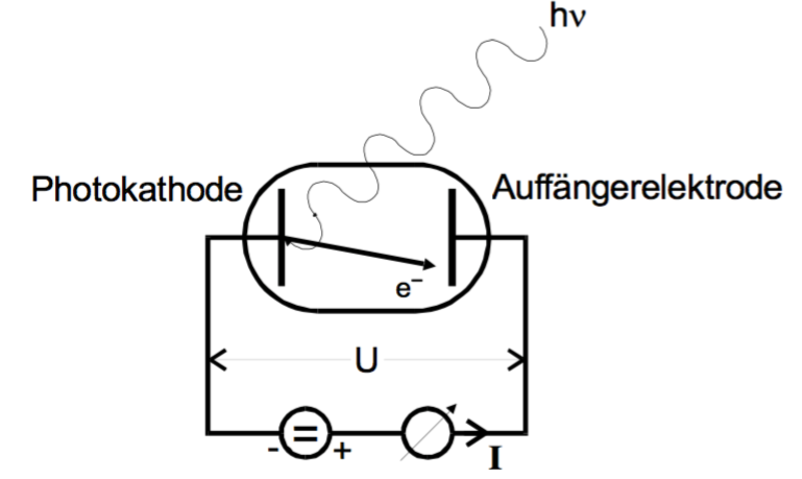
\includegraphics[height = 5cm]{NacktbilderMilaKunis/prinzipaufbau.pdf}
  \caption{Prinzipieller Aufbau zur Untersuchung des Photoeffekts\cite{anleitung}.}
  \label{fig:prinzipaufbau}
\end{figure}

\begin{enumerate}
  \item Die Lichtintensität hat keinen Einfluss auf die kinetische Energie
  der Elektronen. Letztere ist proportional zur Lichtfrequenz.
  \item Unterhalb einer bestimmten Grenzfrequenz können die Photonen
  keine Elektronen mehr auslösen.
  \item Proportional zur Lichtintensität steigt die Zahl der pro Zeiteinheit
  ausgelösten Elektronen.
\end{enumerate}

Die ersten Beiden lassen sich anhand von Gleichung \eqref{eqn:energiebilanz}
erklären. Die auftreffenden Photonen lösen die Elektronen aus der Metalloberfläche aus.
Dabei besitzen sie die Energie $E_\text{Photon} = h \nu$; diese wird
auf die Elektronen übertragen. Ein Teil wird dabei benötigt um die Elektronen
auszulösen: die Austrittsarbeit $A_\g{k}$. Der Rest geht in die kinetische Energie
des Elektrons über.
Also hat nur die Lichtfrequenz einen Einfluss auf die kinetische Energie
des Elektrons.
Auch ist zu verstehen, dass die Austrittsarbeit eine Grenzfrequenz festlegt, die
das Photon überschreiten muss, um Elektronen auslösen zu können.
\begin{equation}
  h \nu = E_\text{kin} + A_\g{k}
  \label{eqn:energiebilanz}
\end{equation}

Da jedes Photon nur ein Elektron auslösen kann, erhöht die Lichtintensität
die Anzahl an ausgelösten Elektronen.

\subsection{Gegenfeldmethode}
\label{sec:gegenfeld}

\begin{figure}[H]
  \centering
  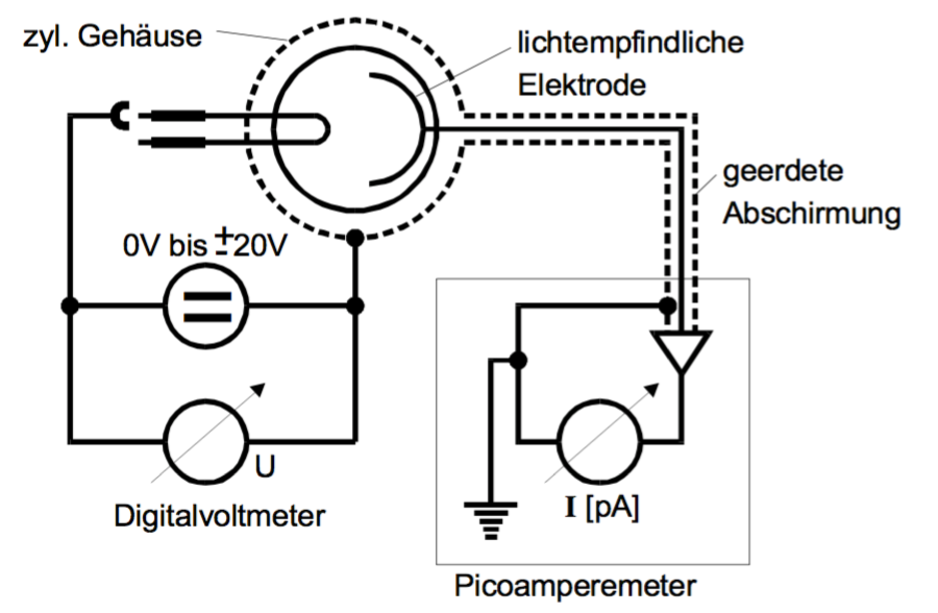
\includegraphics[height = 6cm]{NacktbilderMilaKunis/elektrikaufbau.pdf}
  \caption{Elektrisches Schaltbild der Messapparatur\cite{anleitung}.}
  \label{fig:elektrikaufbau}
\end{figure}

In Abbildung \ref{fig:elektrikaufbau} ist die elektrische Schaltung bei Bestimmung
der kinetischen Energie der Elektronen mit der Gegenfeldmethode gezeigt.
Hierbei wird an die Anode und Kathode eine variable Gegenspannung $U_\g{g}$
so angelegt, dass keine Elektronen mehr die Anode erreichen, da sie vollständig
abgebremst werden.
Hier gilt:
\begin{equation}
  e_0 U_\g{g} = \frac{1}{2} m_0 v_\text{max}^2.
\end{equation}
Demnach ergibt sich eingesetzt in Gleichung \eqref{eqn:energiebilanz}:
\begin{equation}
  h \nu = e_0 U_\g{g} + A_\g{k}.
  \label{eqn:gegenfeld}
\end{equation}
Damit lässt sich also nach der entsprechenden Messreihe das Verhältnis von Wirkungsquantum
zur Elementarladung bestimmen.

Allerdings muss beachtet werden, dass der Strom mit der Bremsspannung nur
langsam gegen Null geht. Zu sehen ist das in Abbildung \ref{fig:bremsspannung}.
Dies liegt daran, dass die austretenden Elektronen auf Grund der Energie die
sie bereits im Festkörper besitzen, eine Energieverteilung aufweisen.
Sie wird durch die Fermi-Dirac-Statistik beschrieben.
Demnach erstreckt sie sich von Null bis zur Fermi-Energie $\zeta$.

\begin{figure}[H]
  \centering
  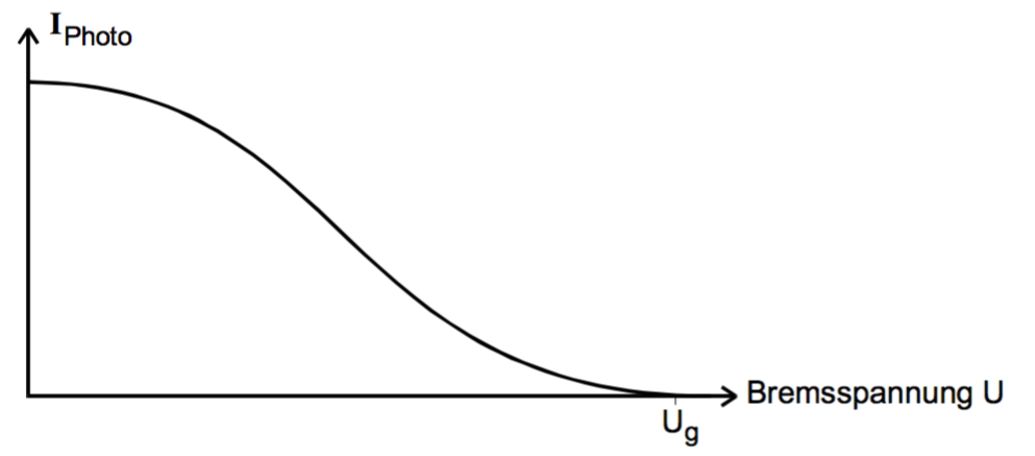
\includegraphics[height = 5cm]{NacktbilderMilaKunis/bremsspannung.pdf}
  \caption{Photostrom in Abhängigkeit von der Bremsspannung\cite{anleitung}.}
  \label{fig:bremsspannung}
\end{figure}

Die Methode zur Bestimmung von $U_\g{g}$ ist die Folgende.
Es wird $\sqrt{I}$ gegen $U$ aufgetragen und $U_\g{g}$ als
Nullstelle der so enstandenen Geraden abgelesen.

Eine weiterer Grund dafür, dass Photonen möglicherweise die Anode nicht erreichen
kann sein, dass die Austrittsarbeit der Anode zu groß ist.
Wenn also $h \nu < A_\g{A}$
gilt, muss eine Beschleunigungsspannung $U_b$ angelegt werden um Strom zu messen, so dass:
\begin{equation*}
  h \nu + e_0 U_\g{b} \geq A_\g{A}.
\end{equation*}
So kann das Elektron die Anode trotz eines zu niedrigen Fermi-Niveaus der Kathode
erreichen. Die Potentialverhältnisse vor und nach Anlegen einer
Beschleunigungsspannung sind in den Abbildungen \ref{fig:potentialverhaeltnisse}\subref{fig:potentialohneub}
und \ref{fig:potentialverhaeltnisse}\subref{fig:potentialmitub} zu sehen.

\begin{figure}[H]
  \centering
  \begin{subfigure}{0.48\textwidth}
    \centering
    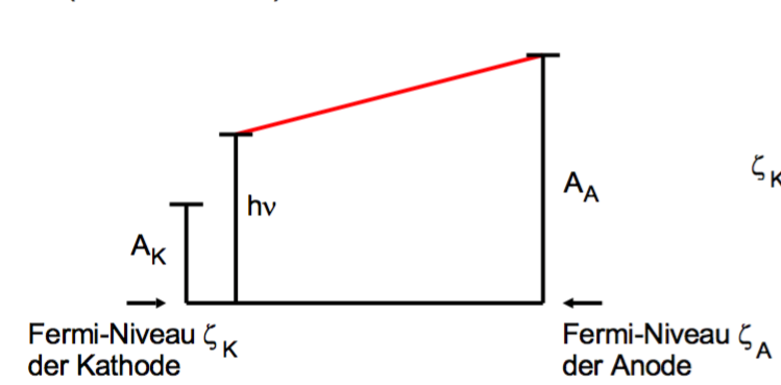
\includegraphics[width = \textwidth]{NacktbilderMilaKunis/potentialohneub.pdf}
    \caption{Potentialverhältnisse zwischen Anode unter Kathode
    unter Berücksichtigung von deren Austrittsarbeiten\cite{anleitung}.}
    \label{fig:potentialohneub}
  \end{subfigure}
  \begin{subfigure}{0.48\textwidth}
    \centering
    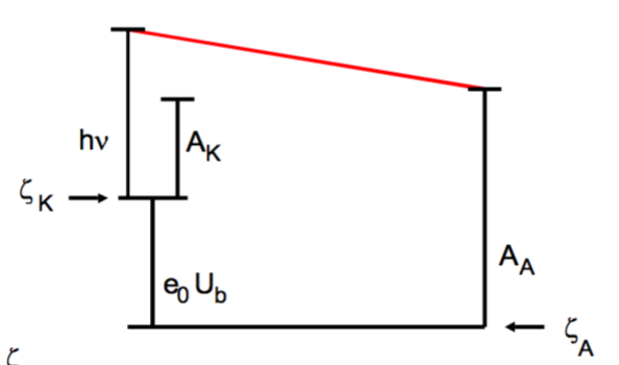
\includegraphics[width = \textwidth]{NacktbilderMilaKunis/potentialmitub.pdf}
    \caption{Potentialverhältnisse nach Anlegen einer Beschleunigungsspannung\cite{anleitung}.}
    \label{fig:potentialmitub}
  \end{subfigure}
  \caption{Potentialverhältnisse der Anode und Kathode mit und ohne Beschleunigungsspannung.}
  \label{fig:potentialverhaeltnisse}
\end{figure}
